% !TEX encoding = UTF-8 Unicode
\documentclass{beamer}

\usepackage[utf8]{inputenc}

\usetheme[navigation]{UMONS}

\title{Pas si élémentaire\dots~mon cher Watson}
\subtitle{Une enquête au cœur de l'histoire des sciences}
\author{Antoine Brandelet$^1$, Ludovic Ducobu$^2$ et Sébastien Gamrath$^3$}
\date{\vspace{-10ex}}

\institute[FS]{%
  Faculté des Sciences\\
  Université de Mons \\
  1 Philosophie et Histoire des Sciences \\
  2 Physique théorique et mathématique \\
  3 Physique Atomique et Astrophysique
  \\[2ex]
  \includegraphics[height=5ex]{UMONS}\hspace{2em}%
  \raisebox{-1ex}{\includegraphics[height=10ex]{UMONS_FS}}
  \\
  \vspace{2ex}
}


\usefonttheme[onlymath]{serif}

\usepackage{multirow}

\usepackage{tikz}
\usetikzlibrary{decorations.pathmorphing,patterns,backgrounds}

\definecolor{vert}{rgb}{0,0.6,0}
\definecolor{rouge}{rgb}{0.7,0,0}



\newcommand{\caneva}[3]{
\draw[color=#3] (-#1/2,-#2/2) -- ++ (0,#2) -- ++ (#1,0) -- ++ (0,-#2) -- cycle;

}

\newcommand{\boule}[2][1]{
  \draw[style={fill=#2}] (0,0) circle(#1);
}

\begin{document}


\begin{frame}
\frametitle{Paradoxe de Galilée}

\framesubtitle{\textit{Galileo Galilei} (1564 P.C. - 1642 P.C.)}

\textit{\textbf{Question :}}

Entre deux objets de masses différentes, lequel tombe le plus vite ?

(Le plus lourd ou le plus léger ?)

\onslide<2->{\vspace{1cm}
\textit{\textbf{Réponse :}}

``C'est l'objet le plus lourd qui tombe le plus vite.''

\textit{Aristote} (384 A.C. - 322 A.C.)}

\phantom{\vspace{1cm}}
\phantom{\textit{\textbf{Objection :}}}

\phantom{``Est-ce que quelqu'un aurait un morceau de ficelle ?''}

\phantom{$\approx$\textit{Galileo Galilei} (1564 P.C. - 1642 P.C.)}

\end{frame}


\begin{frame}
\begin{center}

\begin{tikzpicture}[background rectangle/.style={fill=cyan}, show background rectangle]
\caneva{5}{8}{cyan}

\only<1>{
\begin{scope}[xshift=-1cm,yshift=3.5cm]
\boule[0.2]{brown}
\draw (0,0) node {\tiny $m_1$};
\end{scope}

\begin{scope}[xshift=1cm,yshift=3.5cm]
\boule[0.4]{brown}
\draw (0,0) node {\scriptsize $m_2$};
\end{scope}
}

\only<2>{
\begin{scope}[xshift=-1cm,yshift=3.cm]
\boule[0.2]{brown}
\draw (0,0) node {\tiny $m_1$};
\end{scope}

\begin{scope}[xshift=1cm,yshift=2.5cm]
\boule[0.4]{brown}
\draw (0,0) node {\scriptsize $m_2$};
\end{scope}
}

\only<3>{
\begin{scope}[xshift=-1cm,yshift=2cm]
\boule[0.2]{brown}
\draw (0,0) node {\tiny $m_1$};
\end{scope}

\begin{scope}[xshift=1cm,yshift=0.5cm]
\boule[0.4]{brown}
\draw (0,0) node {\scriptsize $m_2$};
\end{scope}
}

\only<4>{
\begin{scope}[xshift=-1cm,yshift=1cm]
\boule[0.2]{brown}
\draw (0,0) node {\tiny $m_1$};
\end{scope}

\begin{scope}[xshift=1cm,yshift=-1.5cm]
\boule[0.4]{brown}
\draw (0,0) node {\scriptsize $m_2$};
\end{scope}
}

\end{tikzpicture}

\end{center}
\end{frame}

\begin{frame}
\frametitle{Paradoxe de Galilée}

\framesubtitle{\textit{Galileo Galilei} (1564 P.C. - 1642 P.C.)}

\textit{\textbf{Question :}}

Entre deux objets de masses différentes, lequel tombe le plus vite ?

(Le plus lourd ou le plus léger ?)

\vspace{1cm}
\textit{\textbf{Réponse :}}

``C'est l'objet le plus lourd qui tombe le plus vite.''

\textit{Aristote} (384 A.C. - 322 A.C.)

\onslide<2->{\vspace{1cm}
\textit{\textbf{Objection :}}

``Est-ce que quelqu'un aurait un morceau de ficelle ?''

$\approx$\textit{Galileo Galilei} (1564 P.C. - 1642 P.C.)}

\end{frame}

\begin{frame}
\begin{center}

\begin{tikzpicture}[background rectangle/.style={fill=cyan}, show background rectangle]

\only<1>{
\caneva{5}{6.8}{cyan}
\begin{scope}[yshift=3.5cm, color=cyan]
\coordinate (A) at (-1,-0.2);
\coordinate (B) at (1,0.4);
\draw (A) .. controls +(0,-0.7) and  +(0,0.7).. (B);
\end{scope}

\begin{scope}[xshift=-1cm,yshift=3.5cm]
\boule[0.2]{brown}
\draw (0,0) node {\tiny $m_1$};
\end{scope}

\begin{scope}[xshift=1cm,yshift=3.5cm]
\boule[0.4]{brown}
\draw (0,0) node {\scriptsize $m_2$};
\end{scope}
}


\only<2>{
\caneva{5}{6.8}{cyan}
\begin{scope}[yshift=3.5cm]
\coordinate (A) at (-1,-0.2);
\coordinate (B) at (1,0.4);
\draw (A) .. controls +(0,-0.7) and  +(0,0.7).. (B);
\end{scope}

\begin{scope}[xshift=-1cm,yshift=3.5cm]
\boule[0.2]{brown}
\draw (0,0) node {\tiny $m_1$};
\end{scope}

\begin{scope}[xshift=1cm,yshift=3.5cm]
\boule[0.4]{brown}
\draw (0,0) node {\scriptsize $m_2$};
\end{scope}
}

\only<3>{
\caneva{5}{7.4}{cyan}
\begin{scope}[yshift=3.7cm,color=cyan]
\coordinate (A) at (-1,-0.2);
\coordinate (B) at (1,-0.1);
\draw (A) .. controls +(0,-0.7) and  +(0,0.7).. (B);
\end{scope}

\begin{scope}[yshift=3.cm]
\coordinate (A) at (-1,-0.2);
\coordinate (B) at (1,-0.1);
\draw (A) .. controls +(0,-0.7) and  +(0,0.7).. (B);
\end{scope}

\begin{scope}[xshift=-1cm,yshift=3.cm]
\boule[0.2]{brown}
\draw (0,0) node {\tiny $m_1$};
\end{scope}

\begin{scope}[xshift=1cm,yshift=2.5cm]
\boule[0.4]{brown}
\draw (0,0) node {\scriptsize $m_2$};
\end{scope}
}

\only<4>{
\caneva{5}{8}{cyan}
\begin{scope}[yshift=2cm]
\coordinate (A) at (-1,-0.2);
\coordinate (B) at (1,-1.1);
\draw (A) .. controls +(0,-0.7) and  +(0,0.7).. (B);
\end{scope}

\begin{scope}[xshift=-1cm,yshift=2cm]
\boule[0.2]{brown}
\draw (0,0) node {\tiny $m_1$};
\end{scope}

\begin{scope}[xshift=1cm,yshift=0.5cm]
\boule[0.4]{brown}
\draw (0,0) node {\scriptsize $m_2$};
\end{scope}
}

\only<5->{
\caneva{5}{8}{cyan}
\begin{scope}[yshift=1cm]
\coordinate (A) at (-1,-0.2);
\coordinate (B) at (1,-2.1);
\draw (A) .. controls +(0,-0.2) and  +(0,0.2).. (B);
\end{scope}

\begin{scope}[xshift=-1cm,yshift=1cm]
\boule[0.2]{brown}
\draw (0,0) node {\tiny $m_1$};
\end{scope}

\begin{scope}[xshift=1cm,yshift=-1.5cm]
\boule[0.4]{brown}
\draw (0,0) node {\scriptsize $m_2$};
\end{scope}
}

\only<6>{\draw (0.,0.) node[above] {\color{red} $?$};}

\end{tikzpicture}

\end{center}
\end{frame}

\begin{frame}
\frametitle{Paradoxe de Galilée}

\framesubtitle{\textit{Galileo Galilei} (1564 P.C. - 1642 P.C.)}

\vspace{-8mm}
\begin{center}
``C'est l'objet le plus lourd qui tombe le plus vite.''
\end{center}

L'objet $2$ (de masse $m_2$) est plus lourd que l'objet $1$ (de masse $m_1$).

$\Rightarrow$ L'objet $2$ tombe plus vite que l'objet $1$.

\onslide<2->{$\Rightarrow$ La ficelle va se tendre et, comme l'objet de masse $m_1$ tombe moins vite, il va freiner l'objet de masse $m_2$.}

\onslide<3->{$\Rightarrow$ Le système (objet $1$ + objet $2$) tombe \emph{moins vite} que l'objet $2$ seul.}

\onslide<4->{\vspace{2mm}
\textbf{\MakeUppercase{Oui mais}}
\vspace{2mm}}

\onslide<5->{Une fois la ficelle tendue, le système (objet $1$ + objet $2$) se déplace comme un seul objet de masse $m_1 + m_2$.

$\Rightarrow$ Le système est plus lourd que l'objet $2$ seul.

$\Rightarrow$ Le système (objet $1$ + objet $2$) tombe \emph{plus vite} que l'objet $2$ seul.}

\end{frame}

\begin{frame}
\frametitle{Paradoxe de Galilée}

\framesubtitle{\textit{Galileo Galilei} (1564 P.C. - 1642 P.C.)}

Autrement dit \dots

Si les objets plus lourds tombent \emph{plus vite} que les objets plus légers, \textbf{alors} les objets plus lourds tombent \emph{moins vite} que les objets plus légers.

\onslide<2->{\vspace{2mm}
Qu'est-ce que \dots~quoi ?}

\onslide<3->{\begin{center}
  \Large Impossibilité logique !
%
  %(Résultat absurde)
\end{center}}

\end{frame}

\begin{frame}
\frametitle{Paradoxe de Galilée : Solution}

\framesubtitle{\textit{Galileo Galilei} (1564 P.C. - 1642 P.C.)}

Comment résoudre ce ``paradoxe'' ?

\begin{itemize}
\onslide<2->{\item[$\hookrightarrow$] L'hypothèse d'Aristote mène à un résultat contradictoire (absurde)

\item[$\Rightarrow$] On \textbf{ne} peut \textbf{pas} considérer que de deux objets, le plus lourd est celui qui tombe le plus vite}

\onslide<3->{\item[$\hookrightarrow$] L'hypothèse inverse mène à la même contradiction

\item[$\Rightarrow$] On \textbf{ne} peut \textbf{pas} non plus considérer que de deux objets, le plus léger est celui qui tombe le plus vite}

\onslide<4->{\item[$\hookrightarrow$] Seule solution : Tous les objets tombent à la même vitesse, indépendement de leur masse.}

\end{itemize}

\onslide<5->{En fait, le ``paradoxe de Galilée'' est une \textbf{preuve par l'absurde} du fait que tous les objets tombent à la même vitesse, indépendement de leur masse.}

\end{frame}



\end{document}
